\begin{frame}{Rezultati simulacije}
\section{Rezultati simulacije}
\begin{itemize}
    \item Simulacijo smo izvedli pri 10,000 točkah\\
    \item Kot rešitev smo dobili izpisano oceno napake ter velikost odstopanja od realne vrednosti:\\
    \item Ocena $\pi$: 3.157200 \\
          Napaka: 0.015607
\end{itemize}
\begin{columns}
    \begin{column}{0.6\textwidth} 


     \begin{figure}
    \centering
     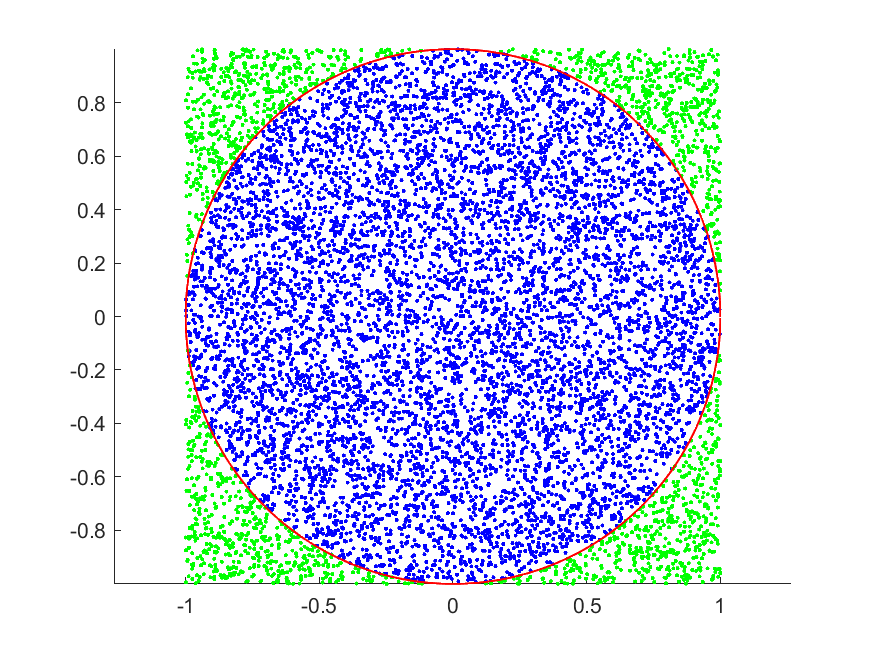
\includegraphics[width=7cm]{rezultat.png}
     \vspace{-2em}
     \caption{Grafični prikaz.}
     \end{figure}

     
    \end{column}
    \begin{column}{0.4\textwidth} 
      Slika prikazuje porazdelitev 10,000 
      naključno generiranih točk.
    \end{column}
  \end{columns}


\end{frame}